\newpage
\section{Abstract}

Diese Dokumentation beschreibt die Entwicklung eines autonomen Fahrzeuges im Projektmodul Pren 1 an der Hochschule Luzern. Das Fahrzeug soll Hindernisse bewältigen und flexibel auf Änderungen in einem vorgegebenen Wegenetz reagieren können (siehe Aufgabenstellung im Anhang \ref{aufgabenstellung}). Ziel ist es, ein Konzept zu entwickeln, das durch technische Innovation und Nachhaltigkeit überzeugt, aber gleichzeitig möglichst robust und einfach aufgebaut ist.
Das Vorgehen umfasst die Erstellung einer umfassenden Anforderungsliste (Kapitel \ref{sec:anforderungsliste}), die Konzeption und Umsetzung eines Simulators (Kapitel \ref{simulator}), die Auswahl geeigneter Technologien aufgrund einer fundierten Technologierecherche (Anhang \ref{technologierecherche}) und schliesslich die Ausarbeitung eines Lösungskonzeptes (Kapitel \ref{lösungskonzept}). Für letzteres wird zu einigen Funktionen Nutzwertanalysen und schliesslich ein Morphologischer Kasten (siehe Anhang \ref{morphologischer kasten}), mit zwei Lösungsansätzen erstellt und ausgewertet. Durchsetzen kann sich das Prinzip Roomba (siehe Abbildung \ref{img:Visualisierung Fahrzeug}). Alle Antriebe werden der Einfachheit halber und aufgrund ihres geringen Gewichtes mit DC-Motoren realisiert. Um die Hindernisbewältigung möglichst simpel zu halten, kommt sie mit einem einzelnen Antrieb aus. Anfangs des Projekts sind die Toleranzen für die Platzierung der Hindernisse seitens der Dozierenden noch sehr hoch, nämlich seitlich 2 cm (siehe Anforderungskatalog in Kapitel \ref{sec:anforderungsliste}), seit dem 25. Oktober ist diese Abweichung nur noch 5 mm. Unser Greifsystem erfüllt nach wie vor die erhöhten Anforderungen, jedoch wäre der Mechanismus einfacher gestaltet worden, wenn die Anforderung von Anfang an einfacher gewesen wäre.
Die Simulation hebt sich ab durch, \textcolor{red}{\textbf{Todo}}. 
Im nächsten Semester im Modul Pren 2 wird das Konzept anhand eines physischen Prototyps umgesetzt und getestet. Als Abschluss findet ein Wettbewerb gegen die übrigen Teams statt, dabei muss die Funktionalität unter Beweis gestellt werden.

\begin{figure}[H] % 'h' steht für here, was bedeutet, dass das Bild möglichst an dieser Stelle eingefügt wird
    \centering
        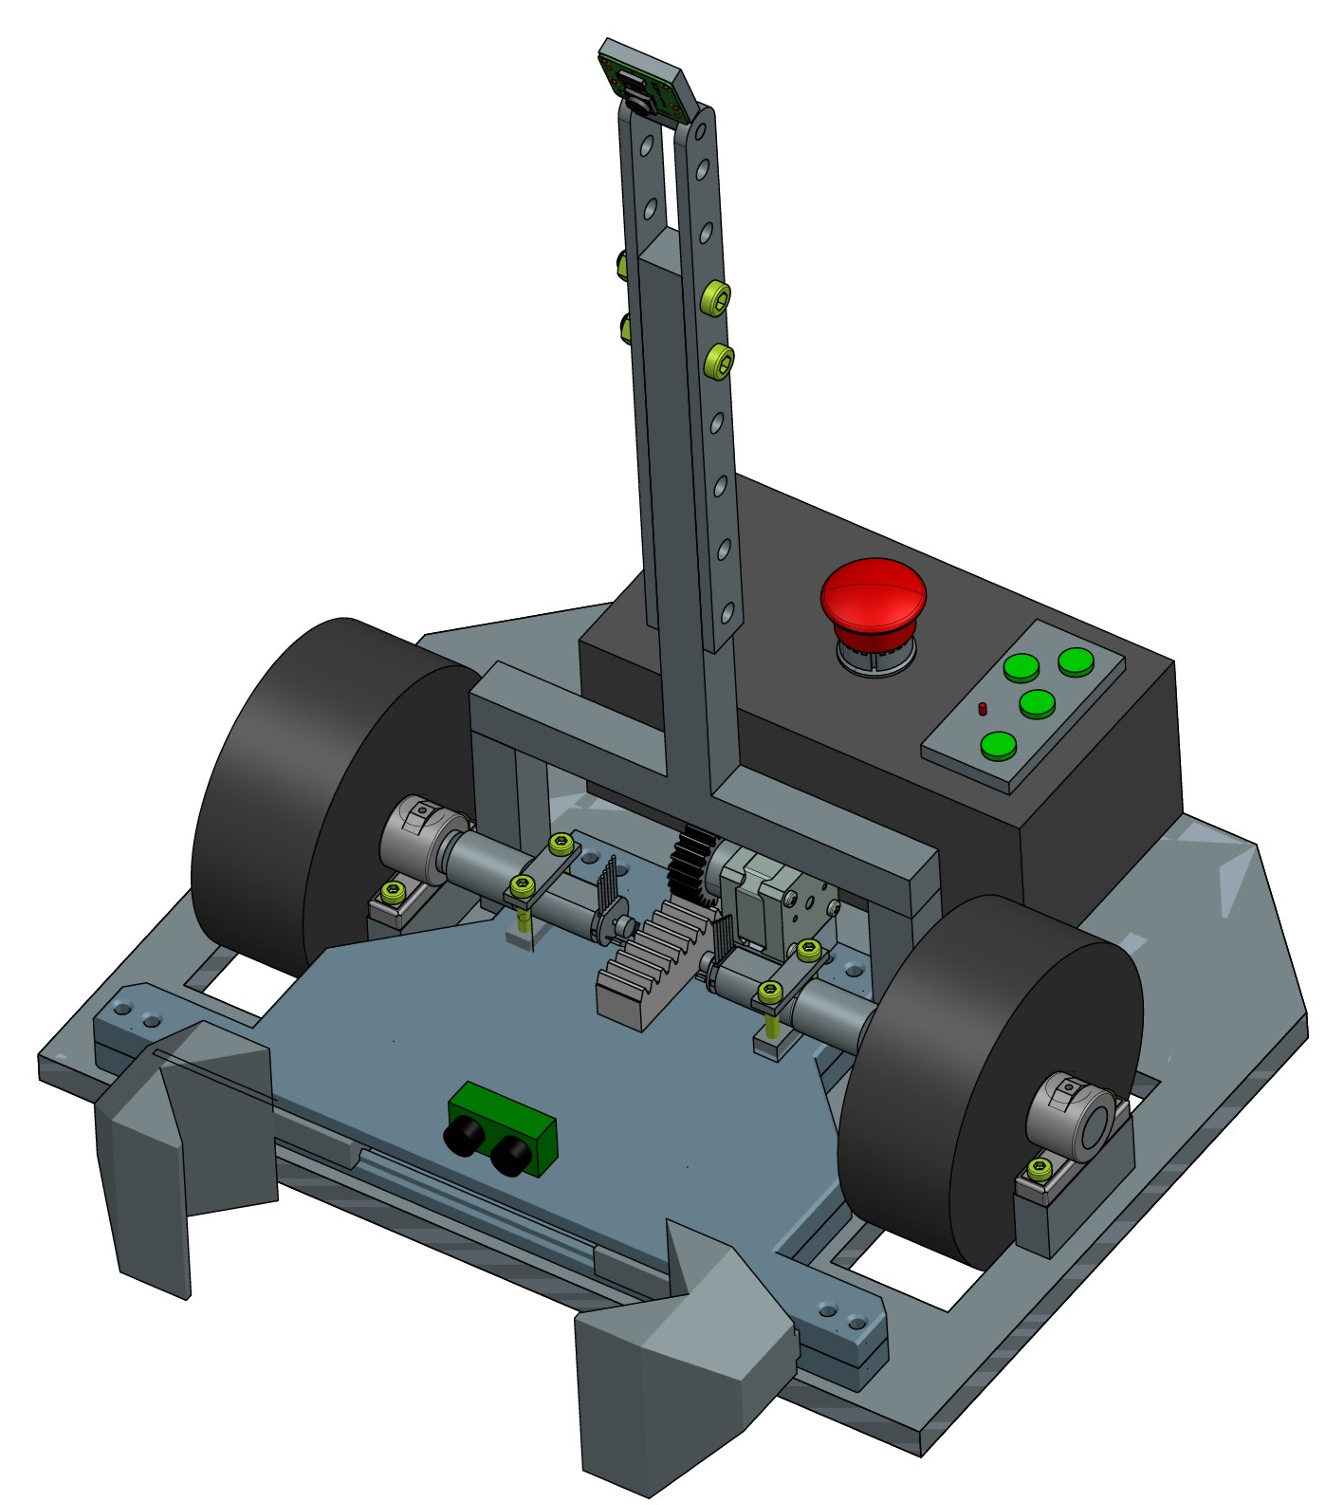
\includegraphics[width=0.5\linewidth]{Skizze_Fahrzeug.png}
        \caption[Visualisierung Fahrzeug]
        {Visualisierung Fahrzeug}
        
        \label{img:Visualisierung Fahrzeug}
    \end{figure} 